\section{Systems description} \label{sec:system}

In this section we describe the tweet classification systems we built. From a module perspective we can describe our systems as composed of three main blocks: text pre-preprocessing (\Cref{subsec:preprocessing}),  text representation (\Cref{subsec:representation}) and classification model (\Cref{subsec:classificationModel}). 


\subsection{Initial investigation} \label{subsec:boh}
To address the tweets classification problem we began our investigation analysing some of the most widely used text representations and classifiers.
In the analysing for possible text representations we began focusing our attention on lexical features based on: \emph{Bag Of Words} \cite{harris1954distributional},\emph{Bag Of N-Grams} (bigrams and trigrams), both with and without \emph{term frequency-inverse document frequency} normalization (i.e., TF-IDF norm).
In relation to classification models that can exploit the above representations,  we analysed \emph{Random Forest, Decision Trees, Support Vector Machines} and \emph{Multi Layer Perceptron}. Since the results obtained with the combination of those \emph{model + representation} were outperformed by neural network based models, we decided not to report their analysis in this paper, but rather focus on the module description of the neural models.


\subsection{Text pre-processing} \label{subsec:preprocessing}
Regarding the text pre-preprocessing, has to be mentioned that the corpus under observation can not be treated as proper written language, because computer-mediated communication (CMC) is highly informal, affecting diamesic\footnote{The variation in a language across medium of communication (e.g. Spanish over the phone versus Spanish over email)} variation with creation of new items supposed to pertain lexicon and graphematic domains \cite{bazzanella2011oscillazioni,cerruti2013netspeak}.
Therefore, in addition to well know pre-processing approach, as stemming (i.e., ST), stopwords (i.e., SW) and punctuation removal (i.e., PR), specific tweets pre-processing techniques has to be taken in consideration.

From previous consideration, we define a set of specific tweet pre-processing approach that take into consideration the following items:
\begin{enumerate*}
\item mentions (i.e., MT),
\item smiley (i.e., SM),
\item emoji (i.e., EM),
\item hashtags (i.e., HT),
\item numbers (i.e., NUM),
\item URL (i.e., URL)
\item and Tweeter reserve-word as RT and FAV (i.e., RW).
\end{enumerate*}

For each of these items we left the possibility to be removed or substituted by constant string (e.g.
\begin{enumerate*}
\item \emph{Pre-processing of @Ambros and \#atoppe :)} $\xrightarrow{substitution} $ \emph{Pre-processing of \$MENTION and \$HASHTAG \$SMILEY},
\item \emph{Pre-processing of @Ambros and \#atoppe :)} $\xrightarrow{removing} $ \emph{Pre-processing of and}
\end{enumerate*}
).

To implement above pre-processing tecnique we took advantage of the following tools:
\begin{enumerate*}
\item NLTK \cite{nltk} and 
\item Preprocessor\footnote{Preprocessor is a preprocessing library for tweet data written in Python, https://github.com/s/preprocessor}.
\end{enumerate*}



\subsection{Text representation} \label{subsec:representation}
The use of neural model suggest us to exploit recent trend over text representation, in particular we decided to use embedding vectors as representation following the approach described by \cite{bojanowski2016enriching}, where tweet elements like \emph{words} and \emph{word n-grams} are represented as vectors of real number with fixed dimension $|v|$.
In this way a whole sentence $s$, with length $|s|$ its number of word, is represented as a \emph{sentence-matrix} $M$ of dimension $|M| = |s| \times |v|$. $|M|$ has to be fixed a priori, therefore $|s|$ and $|v|$ have to be estimated. $|v|$ was fixed to 300 following \cite{bojanowski2016enriching}. $|s|$ was left as a system parameter that after optimization was fixed to $|s| = 30$, with this choice 
input sentences longer than $|s|$ are truncated, while shorter ones are padded with null vectors (i.e., a vector of all zeros).
Depending of chosen tweets elements a different embedding function has to be estimated (i.e., learnt), in the continuation we are going to analyse the possible choices.

\subsubsection{Word embedding.}
Choosing words as elements to be mapped by the embedding function, raise some challenge over the function estimation related to data availability. In our case the available corpus is very small and estimated embeddings could lead to low performance.
To solve this problem, we decided to used a pre-trained embeddings estimated over Wikipedia using a particular approach called \emph{fastText} \cite{bojanowski2016enriching}.

Using this approach, after the sentence-matrix embeddings are calculated, matrix's weights can be set to \emph{static} or \emph{non-static}. In the latter case, backward propagation will be able to adjust its values otherwise they will stay fixed as initially calculated by the embedding function.

In this way four possible combination of sentence-matrix embeddings can be formulated: 
\begin{enumerate*}
\item the use of a pre-trained embedding function (i.e., FastText from Wikipedia) and
\item static or non-static weights.
\end{enumerate*}
From this combination the one composed of static weight without pre-trained embeddings won't be take in consideration for obvious reasons, while we decided to use two pre-trained function from Spanish (i.e., ES) and Catalan (i.e., CA) to see how the use of pre-trained embeddings of a similar language will perform in relation to static/non-static weights.
Meaning that the cases in consideration will be five:
\begin{enumerate*}
\item ES static,
\item CA static,
\item ES non-static,
\item CA non-static,
\item (no pre-trained embeddings) non-static.
\end{enumerate*}

\subsubsection{N-gram embedding.}
Choosing n-grams as element to be mapped by the embedding function, raises more challenges respect simple words, because no pre-trained embeddings are available and in this case the corpus has to be significantly big, otherwise n-gram frequencies will be really low and the estimation algorithm is not able to learn a valid embedding.
Our insight was empirically validated by a very low performance. Nevertheless, as explained in the following, this embedding will be used in a particular model that won't rely its performance just over n-gram embeddings.


\subsection{Classification models} \label{subsec:classificationModel}
Following, we describe the neural models used for the classification module, where for each of them the input layer uses text representations described in \Cref{subsec:representation} (i.e., sentence-matrix).


\subsubsection{Fast text.}
This model was introduced in \cite{joulin2016bag}, where its main difference from our neural model is the use of a particular input layer. In details, rather than using only words or only n-gram as element for the embedding, both elements are embedded with the aim of capturing partial information about words order.
The complete architecture is illustrated in \Cref{fig:fastText}.Here the input layer is directly fed into a \emph{Global Average Pooling} layer, that transforms the sentence-matrix in a single vector, that is projected into two dense layers.
Regarding the architectural references in \cite{joulin2016bag}, they used a number of hidden layers fixed to ten, but we measured better performance using just two layers, moreover we integrate both dropout, gaussian noise and batch normalization.

\begin{figure}[h]
\footnotesize
\centering
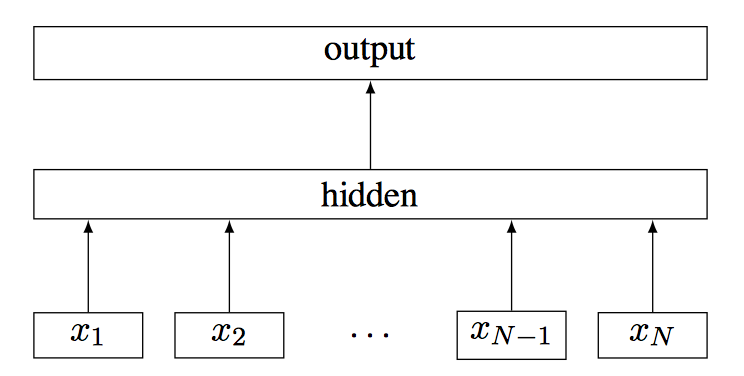
\includegraphics[width=.5\columnwidth]{fast_text}
\caption{\cite{joulin2016bag} Model architecture of \emph{fastText} for a sentence with $N$ n-gram features $x_1,\dots,x_N$. The features are embedded and averaged to form the hidden variable.}
\label{fig:fastText}
\end{figure}


\subsubsection{Convolutional Neural Network.}
Convolutional Neural Networks (CNN) are considered state of the art in many text classification problem. Therefore, we decide to use them in a simple architecture composed by a convolutional layer, followed by a \emph{Global Max Pooling} layer and two dense layers.

\subsubsection{KIM.}
This model was introduced in \cite{kim2014convolutional}. It can be seen as a particular CNN where the convolutional layer has multiple kernels' size and feature maps.
The complete architecture is illustrated in \Cref{fig:kim}, here the input layer (i.e., sentence-matrix) is processed in a convolutional layer of multiple filters with different sizes, each of these results are fed into \emph{Max Pooling} layers and finally the concatenation of them (previously flatten to be dimensional coherent) is projected into a dense layer.
The intuition behind this model is that smaller filter should be able to capture short sentence patterns similar to n-grams, while bigger ones should capture sentence level features.
Regarding the architectural references in \cite{kim2014convolutional}, the number filter $|f|$ and their size was optimized leading to the following results: $|f| = 4, f_1 = 2\times2, f_2 = 3\times3, f_3 = 5\times5, f_4 = 7\times7$.

\begin{figure}[h]
\footnotesize
\centering
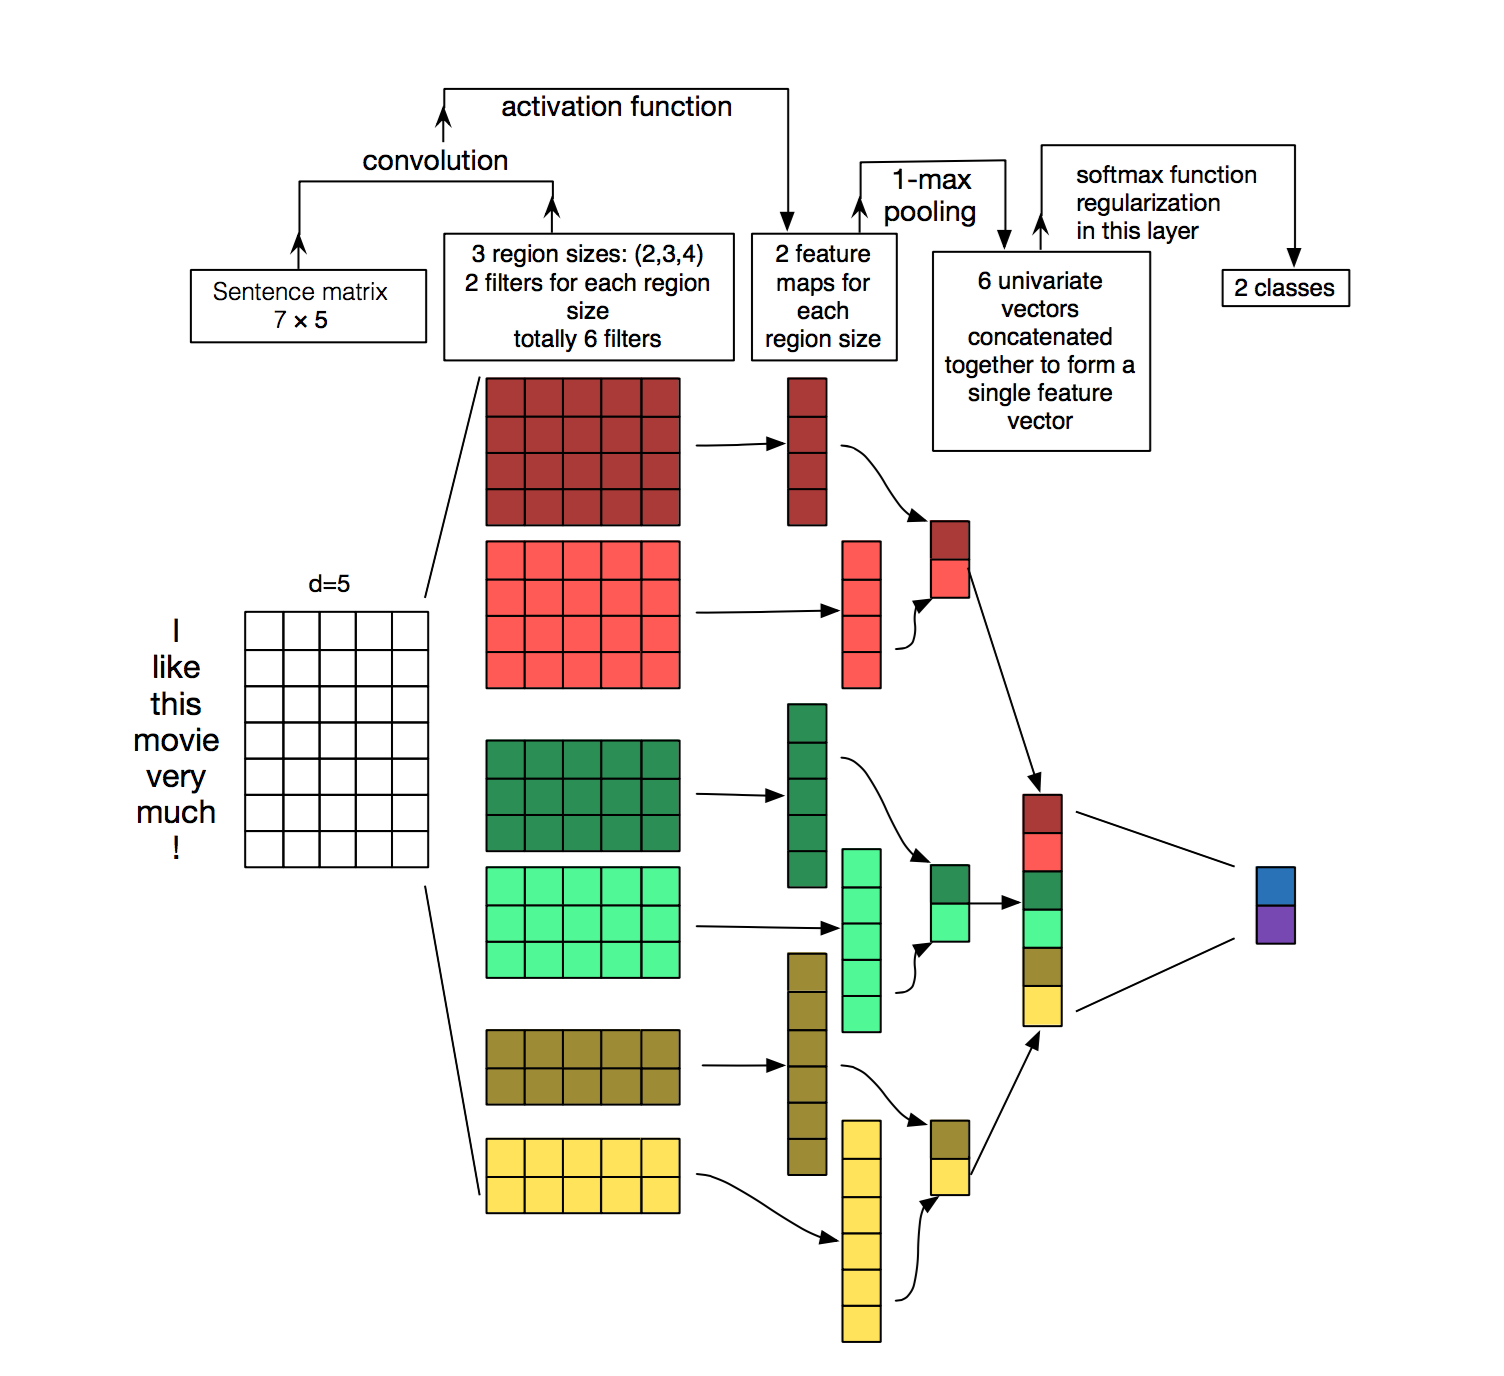
\includegraphics[width=.75\columnwidth]{kim_cnn}
\caption{\cite{zhang2015sensitivity} Illustration of a Convolutional Neural Network (CNN) architecture for sentence classification}
\label{fig:kim}
\end{figure}

\subsubsection{Long short-term memory.}
LSTM is a type of Recurrent Neural Network (RNN) that is relatively insensitive to gap length. Thanks to this behaviour, they are considered state of the art in some NLP problems.
Our architecture was made of an embedded input layer followed by an LSTM layer of 128 units, terminated by a dense layer. Moreover, to avoid overfitting we used dropout and recurrent dropout.

\subsubsection{Bidirectional LSTM.} Similar to the previous model, bidirectional LSTM is a variation of LSTM where the two RNN receive different inputs, the original and its reverse order, and their results are connected through the recurrent layers.
Our architecture follow the previous one with an LSTM layer of 128 units terminating with a dense layer, where all layers used dropout and recurrent dropout.

